\newcommand{\vp}{\vec{p}}
\newcommand{\vq}{\vec{q}}
\newcommand{\vr}{\vec{r}}

\chapter{Vectors}
\label{sec:vectors}

A \myindx{vector} is an ``arrow'' in space given by a starting point and and endpoint. A vector 
has a length and a direction. Since vectors are an important part of the geometry of 
surfaces, the will be introduced briefly here.

\begin{figure}[h]
\begin{center}
  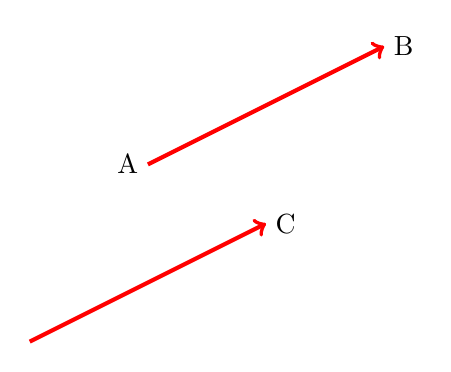
\begin{tikzpicture}[scale=1.5]
    \txfig{0}{0}{3.5}{2.5}
    \coordinate (a) at (1,1.5);    
    \coordinate (b) at (3,2.5);    
    \node[left] at (a) {A} ;
    \node[right] at (b) {B} ;
    \node[right] at (2,1) {C} ;
    \pgfsetlinewidth{1.5pt};
    \draw[->,red] (a) -- (b);
    \draw[->,red] (0,0) -- (2,1);
  \end{tikzpicture}
  \caption{\small The vector from A to B is equivalent to the vector from the 
origin to C, since both have an x-component of 2 and a y-component of 1.}
  \label{fig-vec}
\end{center}
\end{figure}

In figure \ref{fig-vec} is shown three points A,B and C. A vector is drawn from A to B and 
another from the origin O to C. These vectors are identical:

\begin{eqnarray*}
    \overline{AB} = \begin{pmatrix} x_1 - x_0 \\  y_1 - y_0 \end{pmatrix} =&
              \begin{pmatrix} 3 - 1 \\  2.5  - 1.5 \end{pmatrix} =&
              \begin{pmatrix} 2 \\  1 \end{pmatrix} \\
    \overline{OC} = \begin{pmatrix} x_1 - x_0 \\  y_1 - y_0 \end{pmatrix} =&
              \begin{pmatrix} 2 - 0 \\  1  - 0 \end{pmatrix} =&
              \begin{pmatrix} 2 \\  1 \end{pmatrix}
\end{eqnarray*}


\begin{figure}[h]
\begin{center}
  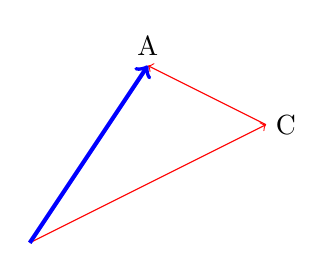
\begin{tikzpicture}[scale=1.5]
    \txfig{0}{0}{3.5}{2.5}
    \coordinate (o) at (0,0);    
    \coordinate (a) at (1,1.5);    
    \coordinate (b) at (3,2.5);    
    \coordinate (c) at (2,1);    
    \node[above] at (a) {A} ;
    \node[right] at (c) {C} ;
    \draw[->,red] (c) -- (a) ;
    \draw[->,red] (o) -- (c);
    \pgfsetlinewidth{1.5pt};
    \draw[->,blue] (o) -- (a);
  \end{tikzpicture}
  \caption{\small The vector $OA$ is equal to the sum of the vectors $OC + CA$.}
\end{center}
\end{figure}

Two vectors can be added by adding the x, and y components, and the same holds for 
subtraction. A vector can be multiplied (or divided) by a factor by multiplying 
(or dividing) each component of the vector by that factor:

$$
     \begin{pmatrix} x_1 \\ y_1 \\ z_1 \end{pmatrix} +
     \begin{pmatrix} x_2 \\ y_2 \\ z_2 \end{pmatrix} 
= \begin{pmatrix} x_1 + x_2 \\ y_1 + y_2 \\ z_1 + z_2 \end{pmatrix}
$$

$$
     a \begin{pmatrix} x \\ y \\ z \end{pmatrix} = \begin{pmatrix} ax \\ ay \\ az \end{pmatrix}
$$

\section{The \myindx{dot product}}

The dot product of two vectors $\vp, \vq$  is defined as 

$$
    \vp\cdot\vq = \begin{pmatrix} p_x \\ p_y \end{pmatrix} \cdot \begin{pmatrix} q_x \\ q_y \end{pmatrix}  
    = p_xq_x + p_yq_y
$$

This is a number (\myindx{scalar}). The value of the dot product is related to the angle $\alpha$ between the two vectors in the 
following way.

$$
   \vp\cdot\vq = |\vp||\vq|\cos\alpha
$$

as a consequence, if two vectors are perpendicular their dot product is zero,
and the dot product of a vector by itself is $\vp\cdot\vp = p_x^2 + p_y^2 = |\vp|^2$


\section{The \myindx{cross product}}
The cross product of two vectors produces a third vector which is perpendicular to 
the two vectors. If 
$$
  \vec{a} =  \begin{pmatrix} a_x \\ a_y \\ a_z \end{pmatrix}, \quad
  \vec{b} =  \begin{pmatrix} b_x \\ b_y \\ b_z \end{pmatrix} \text{then} \qquad
   \vec{a}\times\vec{b} = \begin{pmatrix} 
                             a_yb_z - a_zb_y \\
                             a_zb_x - a_xb_z \\
                             a_xb_y - a_yb_x
                          \end{pmatrix}
$$


Another property of the cross product is that the length of the resultant vector 
is equal to the area spanned by the two vectors.

\section{Formulas for vector products}
Some formulas for dot and cross products and their combinations
\begin{eqnarray*}
    \vp\times\vq & =& -(\vq\times\vp) \\
    \vp\cdot(\vq\times\vr)& =& (\vp\times\vq )\cdot\vr \\
    (\vp\times\vq)\cdot(\vp\times\vq)& =& (\vp\cdot\vp)(\vq\cdot\vq) - (\vp\cdot\vq)^2 \\
    \vp\times(\vq\times\vr)& =& \vq(\vp\cdot\vr) - \vr(\vp\cdot\vq)
\end{eqnarray*}


\myhrule
\begin{myex}
What are the dot products of combinations of these vectors?
$$
  \vec{a} = \begin{pmatrix} -1 \\ 4 \end{pmatrix}, \quad
  \vec{b} = \begin{pmatrix} 2 \\ 1/2 \end{pmatrix}, \quad
  \vec{c} = \begin{pmatrix} 1 \\ -1 \end{pmatrix}
$$
\emph{Answer:}
$$
   \vec{a}\cdot\vec{b} = (-1)\cdot 2 + 4\cdot(1/2) = 0
$$

$$
   \vec{a}\cdot\vec{c} = (-1)\cdot 1 + 4\cdot(-1) = -5
$$

$$
   \vec{b}\cdot\vec{c} = 2\cdot 1 + (1/2)\cdot(-1) = 1.5 
$$
so only the pair $\vec{a}$ and $\vec{b}$ are orthogonal.
\end{myex}


\begin{myex}
What are the length of the vectors $\vec{a}$, $\vec{b}$, and $\vec{c}$ in the 
previous example?
\begin{eqnarray*}
\vec{a}\cdot\vec{a} =& |\vec{a}|^2 =& (-1)\cdot(-1) + 4\cdot4 = 17 \\
\vec{b}\cdot\vec{b} =& |\vec{b}|^2 =& 2\cdot2 + (1/2)\cdot(1/2) = 4.25 \\ 
\vec{c}\cdot\vec{c} =& |\vec{c}|^2 =& 1\cdot1 + (-1)\cdot(-1) = 2 
\end{eqnarray*}
so the lengths of $\vec{a}$, $\vec{b}$, and $\vec{c}$  
are $\sqrt{17}$, $\sqrt{4.25}$ and $\sqrt{2}$. 
\end{myex}


\begin{myex}
If the two vectors
$$
   \vec{a} = \begin{pmatrix} 1 \\ 0 \\ 0 \end{pmatrix},\quad \vec{b} = \begin{pmatrix} 0 \\ 1 \\ 0 \end{pmatrix} ,\quad  \text{then} \qquad
   \vec{a}\times\vec{b} = \begin{pmatrix} 0 \\ 0 \\ 1 \end{pmatrix}
$$
\end{myex}
